\documentclass[class=report, crop=false]{standalone}
\usepackage[subpreambles=true]{standalone}
\usepackage{import}
\usepackage{graphicx}
\begin{document}

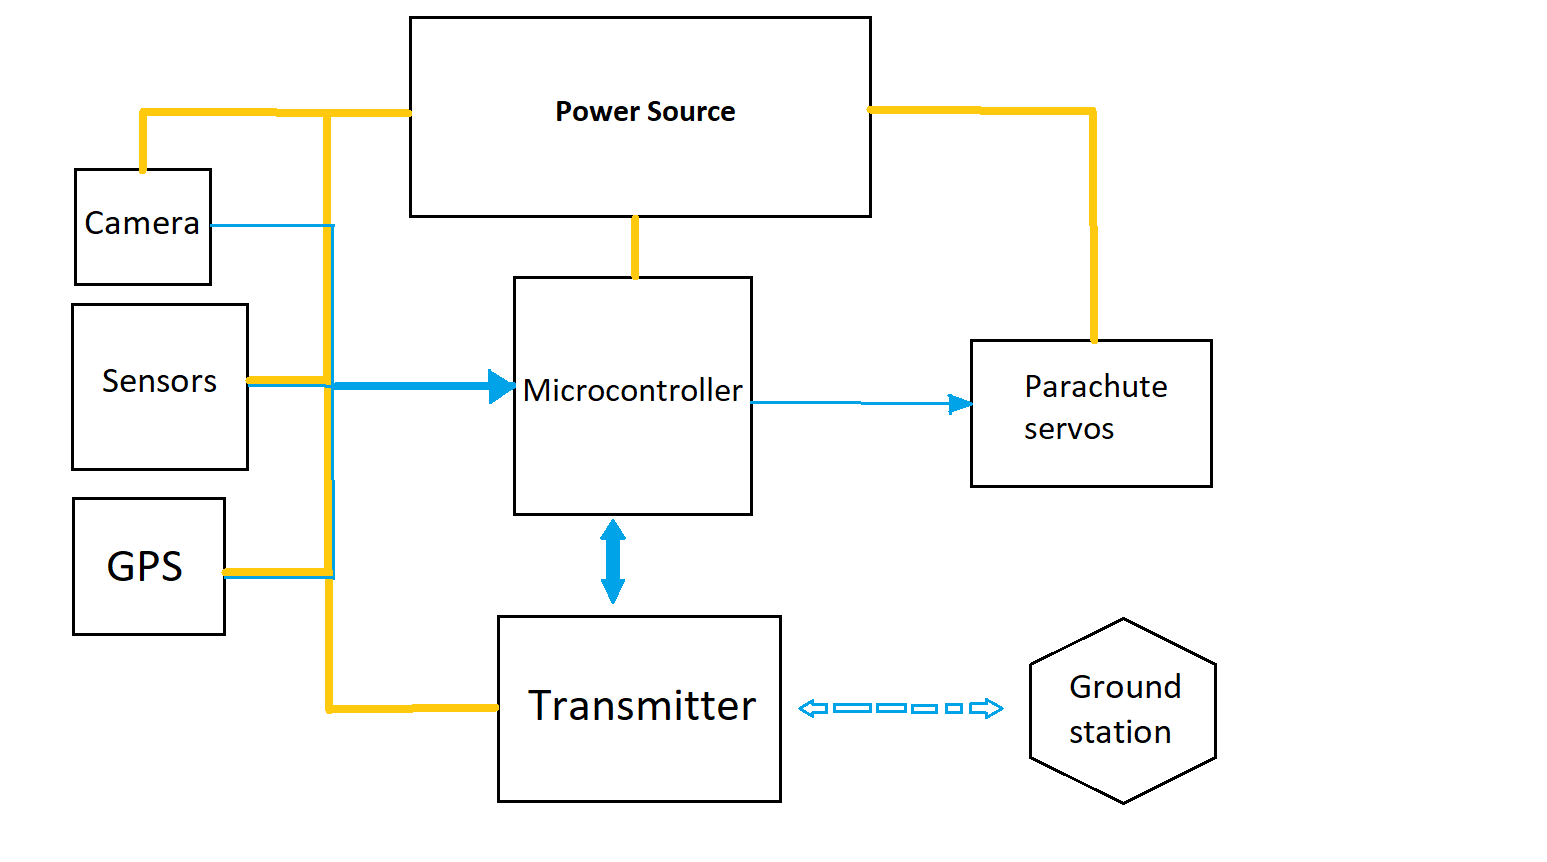
\includegraphics[width=\columnwidth]{ext/electrical1.png} 
\captionof{figure}{A schema of the satellite's electrical design}
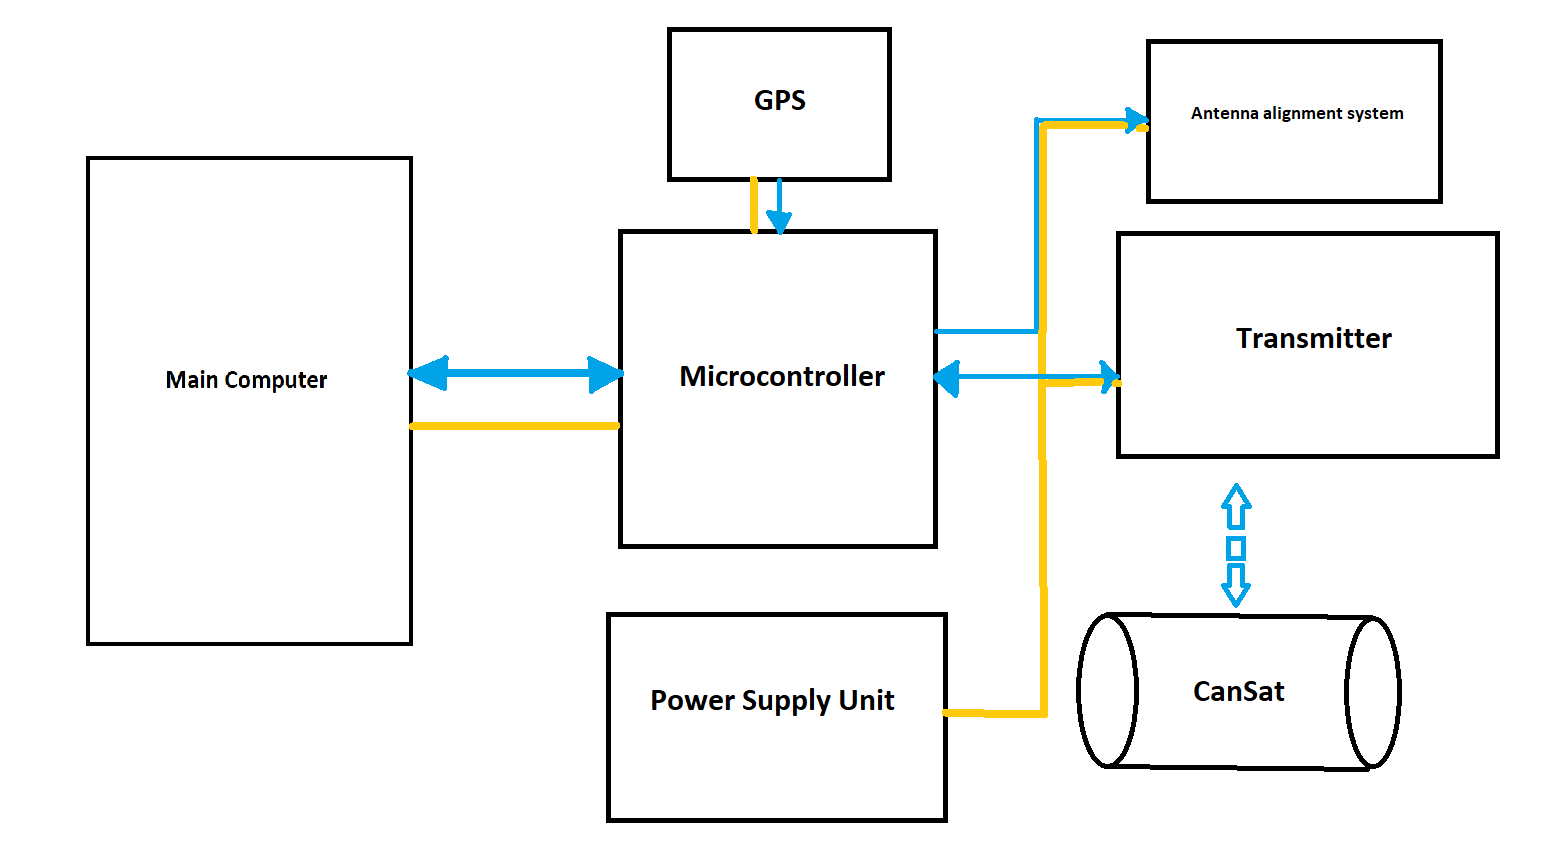
\includegraphics[width=\columnwidth]{ext/electrical2.png} 
\captionof{figure}{A schema of the ground station's electrical design}
\newpage
\subsection*{Primary mission devices}
Primary mission devices (PMDs) are the most essential electronic components of the CanSat. The flaw of any of those components will most likely lead to the failure of the whole program.
The list of all PMDs:
\begin{itemize}
\item On-board computer \\
  The on-board computer is the most important component of the CanSat. It is responsible for collecting data from the sensors, processing them, and transmitting through the radio transmitter module.
  It will also react to data received from the ground station. \\
  We are using the mainboard from the CanSat Kit. Apart from the computer, the mainboard consists of a long-range radio communication component, so no external module is needed.
\item Primary mission sensors \\
  Primary mission sensors shall accomplish the primary mission of the satellite. 
  Carrying them out correctly is required to participate in the CanSat competition. \\
  We are using sensors from the CanSat kit, the LM35 thermistor, and the BMP280 pressure sensor. \\
  The thermistor has a precision of $0.5^{\circ} \text{C}$ and a measurement range from $-55^{\circ} \text{C}$ to $150^{\circ} \text{C}$. \\
  The barometer uncertainty is $1\text{hPa}$ and can measure pressure from $300\text{hPa}$ to $1100\text{hPa}$. 

\item Radio communication module \\
  In order to realize the primary mission, the ground station has to receive readings from satellite sensors every once a second. \\
  To accomplish this task, a long-range communication component will be present onboard the CanSat.
  This task will be performed by an SX1278 transceiver located on the CanSat kit mainboard.
\end{itemize}
\subsection*{Secondary mission components} 

  Secondary mission devices (SMD) are CanSat components needed to fulfill all non-primary missions.
  Unlike PMDs, an error of an SMD might lead to a breakdown of a mission, but not of a whole program.
  The list of all SMDs:
\begin{itemize}
\item GPS receiver \\
  For the SatTrack system to work properly, the ground control requires precise geolocation of the satellite at any given time. \\
  A GPS receiver onboard the satellite provides the current coordinates, while the transmitter sends those coordinates to the ground station. The GPS we are using is MTK3339.
\item Camera \\
  To make the CanSat program more interesting, we plan to record the descent of the satellite with an onboard camera. \\
  For this mission, we equiped our CanSat with an Arducam-Mini OV2640.

\item Parachute steering system \\
  For the GlideCan system to successfully control the movement of the satellite - via manipulating the position of the parachute - a steering system is needed. \\
  The system is planned to consist of a servomotor or servomotors located inside the satellite, which will pull the strings attached to the chute.
  The servomotor we will use is yet to be determined.

\item Power Supply \\
  In order for all electronic subsystems to work, a power supply is needed. The supply has to be compact, reliable, and long-lasting. \\
  We are going to use two Li-Ion batteries with a capacity of $1200$mAh each and a voltage of $\approx 4.2\text{V}$.

\item Additional sensors \\
  Additional sensors are going to provide us with more data, and they help with both the primary and secondary missions.
  These sensors are: a humidity sensor, an accelerometer and a magnetometer.

\end{itemize}


\end{document}
